\subsection{Planes}
\noindent
A plane can also be formed using a point in the plane, $P$, and a vector perpendicular to the plane, $\vec{n}$.
All vectors $\langle x,y,z \rangle$ that originate from $P$ and remain in the plane must be perpendicular to $\vec{n}$, so their dot product with $\vec{n}$ would be 0.
So, the point-normal form of a plane is\footnote{Conventionally, $\vec{n}$ is a unit vector, $\hat{n}$.}
\begin{equation*}
	\vec{n}\cdot\left(\langle x,y,z \rangle - \vec{P}\right) = 0.
\end{equation*}

\begin{figure}[H]
	\centering
	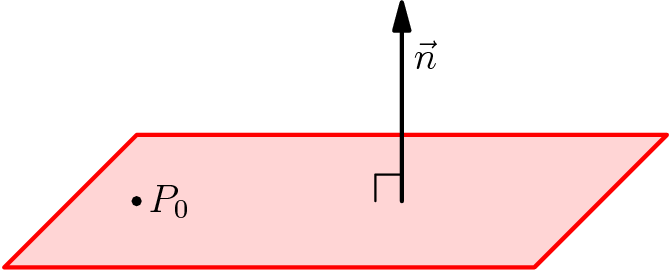
\includegraphics[width=0.5\textwidth]{./vectorValuedFunctions/PlaneNormalVector.png}
	\caption{A point $P_0$ and a normal vector $\vec{n}$ define a plane.}
\end{figure}

\noindent
One can also construct a plane from 3 non-collinear points in the plane.
One can still take advantage of point-normal form here by choosing 1 point to be $P_0$ and drawing vectors from this point to the two other points.
The cross product of these two vectors is $\vec{n}$.
\begin{equation*}
	\left(\left(\vec{P_1} - \vec{P_0}\right) \times \left(\vec{P_2} - \vec{P_0}\right)\right) \cdot \left(\langle x,y,z \rangle - \vec{P_0}\right) = 0,
\end{equation*}
where $P_0$, $P_1$, and $P_2$ are the three points in the plane.\\

\noindent
One can also construct a plane from a point in the plane, $P_0$, and a line in the plane, $\vec{r}(t) = \vec{P_1} + t\vec{v}$, that doesn't pass through $P_0$.
One can get this setup into point-normal form by choosing a an output of $\vec{r}(t)$, like $\vec{P_1}$, and constructing a vector that points from $\vec{P_1}$ to $\vec{P_0}$, $\vec{P_1}-\vec{P_0}$, and crossing this with $\vec{v}$ to find $\vec{n}$.
\begin{equation*}
	\left(\vec{v} \times \left(\vec{P_1} - \vec{P_0}\right)\right) \cdot \left(\langle x,y,z \rangle - \vec{P_0}\right) = 0
\end{equation*}

\noindent
One can also construct a plane from two intersecting lines, $\vec{r_1}(t) = \vec{P_0} + t\vec{v_1}$ and $\vec{r_2}(t) = \vec{P_0} + t\vec{v_2}$, where $P_0$ is where the two lines intersect.
One can cross $\vec{v_1}$ with $\vec{v_2}$ to get the normal vector.
\begin{equation*}
	\left(\vec{v_1} \times \vec{v_2}\right) \cdot \left(\langle x,y,z \rangle - \vec{P}_{0}\right) = 0
\end{equation*}